\titulo{MODELAGEM E CONTROLE DE UM CONVERSOR BOOST CC--CC EM CONDUÇÃO CONTÍNUA} % Titulo em português
\title{MODELLING AND CONTROL OF A DC--DC BOOST CONVERTER IN CONTINUOUS CONDUCTION MODE} % Título em inglês

\maketitle

\editorfootnote{Artigo compilado em {\today} às {\currenttime}h, referente Atividade Prática Supervisionada (APS) da disciplina de Eletrônica de Potência -- ET76C, ministrada pelo Prof. Adriano Ruseler, Dr. Eng.\\
Repositório: \url{https://github.com/AdrianoRuseler/ET76C-APS} }



\begin{resumo}  O resumo deve ser conciso e ao mesmo tempo refletir o que é apresentado no artigo, cujo entendimento deve independer da leitura do trabalho, sem notas de rodapé, abreviações e referências. Deve ser escrito em apenas um parágrafo, de forma impessoal, sem equações ou tabelas. Evite repetir expressões ou utilizar varias vezes a mesma palavra. Busque encadear as frases em um início, meio e fim.
\end{resumo}

\begin{palavraschave }
		Os autores devem apresentar um conjunto de até seis palavras-chave (em ordem alfabética, todas iniciais maiúsculas e separadas por vírgula) que possam identificar os principais tópicos abordados.	
%Use a lista de palavras--chave:\\ \url{http://www.ieee.org/organizations/pubs/ani_prod/keywrd98.txt}	
\end{palavraschave }

\englishtitle

\begin{abstract}
	The abstract must be a concise yet comprehensive reflection of what is in your article, a microcosm of the full article. The abstract must be written as one paragraph, and should not contain displayed mathematical equations or tabular material.  Ensure that your abstract reads well and is grammatically correct.
\end{abstract}

\begin{keywords}
	The abstract should include three or four different keywords or phrases, as this will help readers to find it. It is important to avoid over-repetition of such phrases as this can result in a page being rejected by search engines. For a list of suggested keywords, \url{http://www.ieee.org/organizations/pubs/ani_prod/keywrd98.txt}
\end{keywords}

%\section*{NOMENCLATURA}
%
%\symbolnomenclature{$P$}{Número de polos.}
%\symbolnomenclature{$V_{qd}$}{Componentes $dq$ da tensão de estator.}


% Introdução
\section{INTRODUÇÃO}


A seção de Introdução tem o objetivo geral de apresentar a natureza do problema abordado no trabalho, através de adequada revisão bibliográfica, o propósito e a contribuição do artigo submetido.

A introdução requer uma breve revisão da literatura referente ao tópico de pesquisa. A introdução é então melhor construída como um funil descritivo, começando com temas gerais e focando lentamente no trabalho em questão. Talvez de três a quatro parágrafos sejam necessários. Uma abordagem pode ser começar com um ou dois parágrafos que introduzam o leitor para o estudo de campo geral. Os parágrafos subsequentes então descrevem como um aspecto deste campo poderia ser melhorado. O parágrafo final é essencial. Ele afirma claramente, provavelmente na primeira frase do parágrafo, qual questão experimental será respondida pelo estudo. A hipótese é então indicada. Em seguida, descreve brevemente a abordagem que foi feita para testar a hipótese. Finalmente, uma frase de resumo pode ser adicionada informando como a resposta da sua pergunta vai contribuir para o campo geral de estudo \figref{fig:boost}.

\begin{figure}[!h]
	\centering
	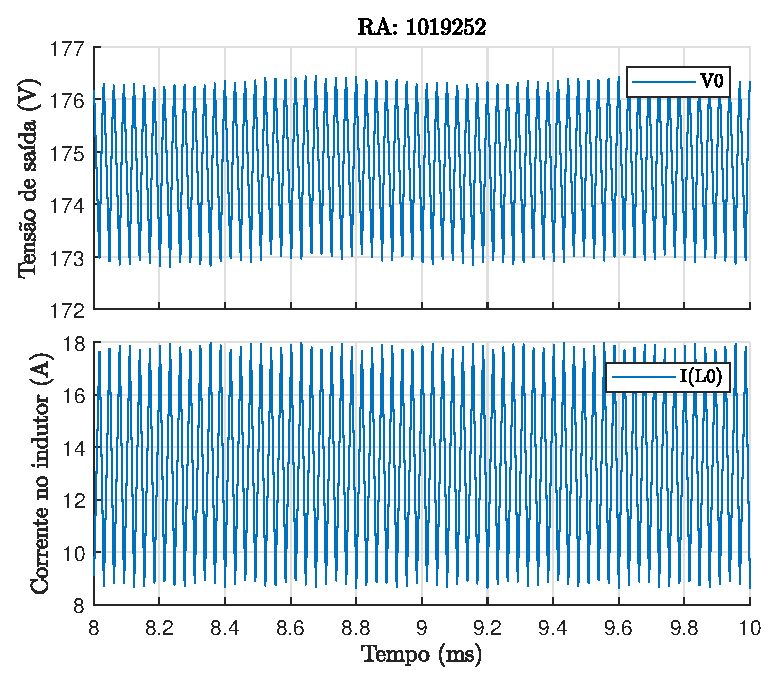
\includegraphics[width=1\linewidth]{Figs/Boost}
	\caption{Conversor Boost.}
	\label{fig:boost}
\end{figure}



\section{Estudo teórico}

Detalhar o projeto do conversor Boost \cite{inep-cccc-2006} no modo de condução contínua (MCC), (ver Planilhas \cite{noauthor_ptc_nodate}).

%\begin{figure*}[!h]
%	\centering
%	\includegraphics[width=0.85\linewidth]{Figs/PWM}
%	\caption{Controlador PI implementado com modulador PWM.}
%	\label{fig:PWM}
%\end{figure*}
%
%
%
%\begin{figure}[!h]
%	\centering
%	\includegraphics[width=0.85\linewidth]{Figs/PWM-PI}
%	\caption{Controlador PI implementado medição de tensão via divisor resistivo.}
%	\label{fig:PI-PWM}
%\end{figure}



\section{Projeto do controlador}

A \tabref{tab:parametrosBoost} apresenta os parâmetros de projeto do conversor Boost.

%\begin{table}[!ht]
%	\centering
\begin{center}
	\captionof{table}{Parâmetros de projeto do conversor Boost}
	\label{tab:parametrosBoost}
	\begin{tabular}{@{}ccc@{}}
		\toprule
		\textbf{Parâmetro} & \textbf{Valor} & \textbf{Símbolo} \\ \midrule			
		Frequência  da rede        & \SI{60}{\hertz}     & $f_0$  \\		
		Frequência de comutação        & \SI{20}{\kilo\hertz}     & $f_s$  \\	
		Tensão contínua de entrada         &  \SI{178}{\V}      & $V_i$  \\
		Tensão contínua de saída         &  \SI{200}{\V}      & $V_0$  \\
		Resistência de carga        & \SI{820}{\ohm}      & $R_0$  \\
			Indutância        & \SI{29.556}{\milli\henry}     & $L_0$  \\
			Capacitor           & \SI{220}{\micro\farad} x \SI{250}{\V}      & $C_0$               \\
%		Razão cíclica de operação       & \SI{35.7142857}{\%}    & $D_{0}$    \\ 
		 \bottomrule	
	\end{tabular}
%\end{table}
\end{center}



%
%\begin{table}[!ht]
%	\centering
%	\caption{Componentes utilizados na montagem do controlador PI}
%	\label{tab:componentesPWM}
%	\begin{tabular}{@{}ccc@{}}
%		\toprule
%		\textbf{Componente} & \textbf{Descrição} & \textbf{Quantidade} \\ \midrule			
%		Resistor  $R_a$     & \SI{100}{\kilo\ohm} -- \SI{1/4}{\W}    & 1    \\	
%		Resistor   $R_b$    & \SI{1.8}{\kilo\ohm} -- \SI{1/4}{\W}    & 1    \\
%		Resistor  $R_{1PI}$     & \SI{390}{\kilo\ohm} -- \SI{1/4}{\W}    & 1     \\	     
%		Resistor  $R_{2PI}$     & \SI{56}{\ohm} -- \SI{1/4}{\W}    & 1   \\  
%	    Capacitor $C_{1PI}$     & \SI{3,9}{\micro\farad} x \SI{25}{\V}      & 1  \\\bottomrule	
%	\end{tabular}
%\end{table}

%



\section{Verificação por simulação}

A análise teórica apresentada anteriormente deve ser verificada por simulação \cite{noauthor_psim_nodate}.
									
 Apresente as formas de onda referentes ao projeto do conversor:
 
\begin{enumerate}
	\item Verificar o comportamento em malha fechada;
\end{enumerate}


\section{Resultados experimentais}


A análise teórica, assim como as simulações, são verificadas de forma definitiva com os resultados experimentais.
\begin{enumerate}									
	\item Verificar o comportamento em malha fechada;
	\item  Apresente uma fotografia do conversor montado;
\end{enumerate}

\section{Conclusões} 


As conclusões devem ser as mais claras possíveis, informando aos leitores sobre a importância do trabalho dentro do contexto em que se situa. As vantagens e desvantagens em relação aos já existentes na literatura devem ser comentadas, assim como os resultados obtidos e as possíveis aplicações práticas do trabalho.


\bibliographystyle{IEEEtran}

\bibliography{Refs/APS} % Inclui arquivos de referência

\balance


